\documentclass[review]{elsarticle}

\usepackage[]{geometry}
\usepackage{amsmath}
\usepackage{amssymb}
\usepackage{graphicx}
\usepackage{xcolor}
\usepackage{hyperref}
\usepackage{natbib}
\bibliographystyle{elsarticle-harv}
\biboptions{authoryear}

\newcommand{\ra}{\rightarrow}
\newcommand{\afs}[2]{\Phi_{#1}^{(#2)}}
\newcommand{\Dfrac}[2]{%
  \ooalign{%
    $\genfrac{}{}{1.2pt}0{#1}{#2}$\cr%
    $\color{white}\genfrac{}{}{.4pt}0{\phantom{#1}}{\phantom{#2}}$}%
}
\newcommand{\cond}{\middle\vert}
\newcommand{\dslash}{/\!\!/}
\newcommand{\Coalc}[4]{\begin{bmatrix}#1\dslash #2 \\ #3\dslash #4 \end{bmatrix}}

\newcommand{\sgcomment}[1]{{\color{red}{SG: #1}}}
\newcommand{\ikcomment}[1]{{\color{blue}{IK: #1}}}
\newcommand{\Var}{\operatorname{Var}}
\journal{Theoretical Population Biology}

\begin{document}
\begin{frontmatter}
  \title{Models of strong selection in large samples. 
  Taming strong selection with large sample sizes.  }

  \author{Ivan Krukov}
  \author{Simon Gravel}

  \begin{abstract}
  The fate of mutations and the genetic load of populations depend on the relative importance of 
  genetic drift and natural selection. In addition, the accuracy of numerical models of evolution
  depends on the strength of both selection and drift: strong selection breaks nearly neutral model assumptions, 
  for example, and strong drift coupled with large sample sizes breaks Kingman's coalescent. 
  
  Thus the regime with strong selection and large sample sizes appears particularly daunting. 
  However, we find that the competition between drift and natural selection in that regime can
  be used to define asymptotically closed recursion equations for the distribution 
  of allele frequencies well beyond the strong selection limit. 
 
  We construct the relevant transition matrices, show how these can
  be used to accurately compute distributions of allele frequencies, and
  discuss the boundaries of this analytically tractable regime. 
  
  Selection becomes more analytically tractable when ...
    
  \ikcomment{This needs to be re-written}
  
    Neutral models of genetic diversity tend to be easier to study than models including selection.
    In the neutral Wright-Fisher model, the number of parental lineages that contribute to ancestry
    of a sample is lower than the number of offspring. As a consequence, useful recursion equations
    can be derived for patterns of polymorphism. By contrast, under negative selection, the number
    of relevant lineages can increase as we go back in time, due to selective deaths. As a result,
    the equivalent recursion equations do not close. However, given a sufficiently large sample
    size, the expected reduction in the number of contributing lineages due to coalescence is larger
    than the increase due to selection, so the net number is unlikely to increase. We use this
    observation to derive asymptotically closed recursion equations for the distribution of allele
    frequencies in finite samples. We show that this approach is accurate under strong drift and
    strong natural selection. We derive several asymptotic results to determine when the sample size
    is sufficiently large for drift to overcome the effect of selection.
  \end{abstract}

\end{frontmatter}

\section{Introduction}
\label{sec:introduciton}

The allele frequency spectrum (\textit{AFS}) is an important summary of genetic diversity that is
commonly used to infer demographic history and natural selection \citep{GutenkunstEtAl2009}. Given a
demographic scenario of population size histories and migrations, the diffusion approximation or
coalescent simulations can be used to obtain a predicted \textit{AFS}. By comparing predictions to
the observed \textit{AFS}, one can compute likelihoods for different demographic scenarios.
Unfortunately, the \textit{AFS} calculations can be time consuming with complex demographic models,
for example with multiple populations, or with large sample sizes.

In the absence of selection, efficient computational shortcuts can be used. Coalescence models such
as \citep{fastsimcoal2, KammEtAl2017} can efficiently compute the \textit{AFS} or subsets of it. In addition,
recursion equations have been derived for moments of the allele frequency distribution
\citep{KimuraCrow1964,Ewens1972,JouganousEtAl2017}. Recently, these recursions have been useful in
fitting complex demographic models to genetic data \citep{JouganousEtAl2017,KammEtAl2017}.
 
In the presence of natural selection, coalescent models become much more complicated, and the
corresponding recursion equations do not close \citep{DonnellyKurtz1999, JouganousEtAl2017} -- they
form an infinite set of coupled ordinary differential equations. Moment-based closure approximations
have been developed \citep{JouganousEtAl2017}, but these are not robust to strong selection and
their convergence properties are not well understood.

Closure of the moment equations under the neutral Wright-Fisher model occurs because the number of
distinct parental lineages that are sampled when drawing $n$ offspring is less than or equal to $n$.
This does not hold under negative selection -- due to selective deaths, the number of parental
lineages that are relevant to a sample of size $n$ can be larger than $n$ \citep{DonnellyKurtz1999a,
  JouganousEtAl2017}. This possible increase is explicit, \textit{e.g.}, in in the ancestral
selection graphs (\textit{ASG}), \citep{KroneNeuhauser1997}.

The actual increase in the number of relevant lineages as we go back in time depends on the relative
importance of drift and selection. Whereas the dynamics of allele frequencies typically depend on
the scaled selection coefficient $Ns$, closure properties depend on the sample size. The number of
in-sample coalescent events per generation is proportional to the square of the sample size $n$,
while the number of selective deaths is linear in $n$. This suggests that with sufficiently large
samples, the effect of selection would be smaller than that of drift, which would prevent the
increase in the number of lineages -- at least most of the times. Thus recursion equations can
become almost-closed, in a sense that we will explore below.

Large sample sizes also bring in the complication of multiple and/or simultaneous coalescent events
\citep{BhaskarEtAl2014}. In this article we derive recursion equations for large sample sizes, and
show that these are asymptotically closed even under strong selection. We show that these transition
matrices can be used to more accurately model the distribution of allele frequencies in moderate to
large samples.

In short, modeling large sample sizes makes it easier to account for strong selection. 

\section{Background}
\label{sec:background}

We consider a haploid Wright-Fisher model with $N$ individuals per generation, focusing on a single
biallelic locus. For a present-day sample with $n_o$ offspring lineages at time $t$, we will be
looking for recursion equations for the allele frequency spectrum, $\afs{n_o}{t}(i_o)$, which we
define as the probability of observing $i_o$ copies of the derived allele in a sample of size $n_o$.
We will do so by considering the process of drawing parental alleles for this finite sample.

\begin{table}
  \centering
  \begin{tabular}{l|p{100mm}}
    Symbol & Meaning\\
    \hline
    $N$ & Population size\\
    $n_p$ & Number of parental lineages\\
    $n_g$ & Number of gametes\\
    $n_o$ & Number of offspring, sample size\\
    $i_p$ & Number of derived alleles in parents\\
    $i_o$ & Number of derived alleles in offspring\\
    $t$ & Time, in generations\\
    $\Phi_{n_o}^{t}(i_o)$ & Allele frequency spectrum in $n_o$ at generation $t$\\
    $s$ & Selection advantage of the derived allele\\
    $x_p$ & Frequency of derived allele in parental generation\\
    $i_o \dslash n_o$ & A sample with $i_o$ derived alleles ``out of'' $n_o$ total\\
    $\mathbf{H}\Coalc{i_p}{n_p}{i_o}{n_o}$ & Hypergeometric probability -
                                             sample $i_o \dslash n_o$ in offspring from $i_p \dslash n_p$ in parental generation\\
    $\mathbf{T}_{r}\Coalc{i_p}{n_p}{i_o}{n_o}$ & Probability of transition from $i_p \dslash n_p$ in parents
                                                 to $i_o \dslash i_o$ in offspring, with $r$ selective events -
                                                 see text for a more detailed description\\
  \end{tabular}
  \caption{\label{tab:symbols} Table of symbols}
\end{table}

Under neutral evolution, each offspring picks a lineage at random with replacement, and the number
$n_p$ of distinct parental lineages is smaller than $n_o$ (Fig.\ref{fig:schematic}A).

To model selection as part of our sampling process, we consider that a parental lineage carrying a derived allele 
is `rejected' as a result of selective death with probability $s>0$
(Fig. \ref{fig:schematic}B, capped line). In such case, we keep sampling until a successful draw.  
This is equivalent to the usual formulation of the Wright-Fisher model: the probability of drawing 
the derived allele is $1-s$ times the probability of drawing the ancestral allele. 
Because the drawing process depends on the state of both selected and rejected alleles, 
the AFS in the offspring will depend on the state of the $n_p$ distinct parents that were sampled,
whether or not they contributed. Because of rejection, $n_p$ can be larger than $n_o.$

To disentangle the effects of drift and selection, we may also make explicit the number of gametes
sampled in the process, $n_g$ (Fig. \ref{fig:schematic}C). The difference $n_g-n_o$ depends only on the
number of selective deaths, $n_g-n_o \ge 0$. The difference $n_p-n_g$ depends only on
coalescence events, $n_p-n_g \le 0$.

We will use this model with $n_g$ in section
\ref{sec:asympt}.

\begin{figure}[h]
  \centering
  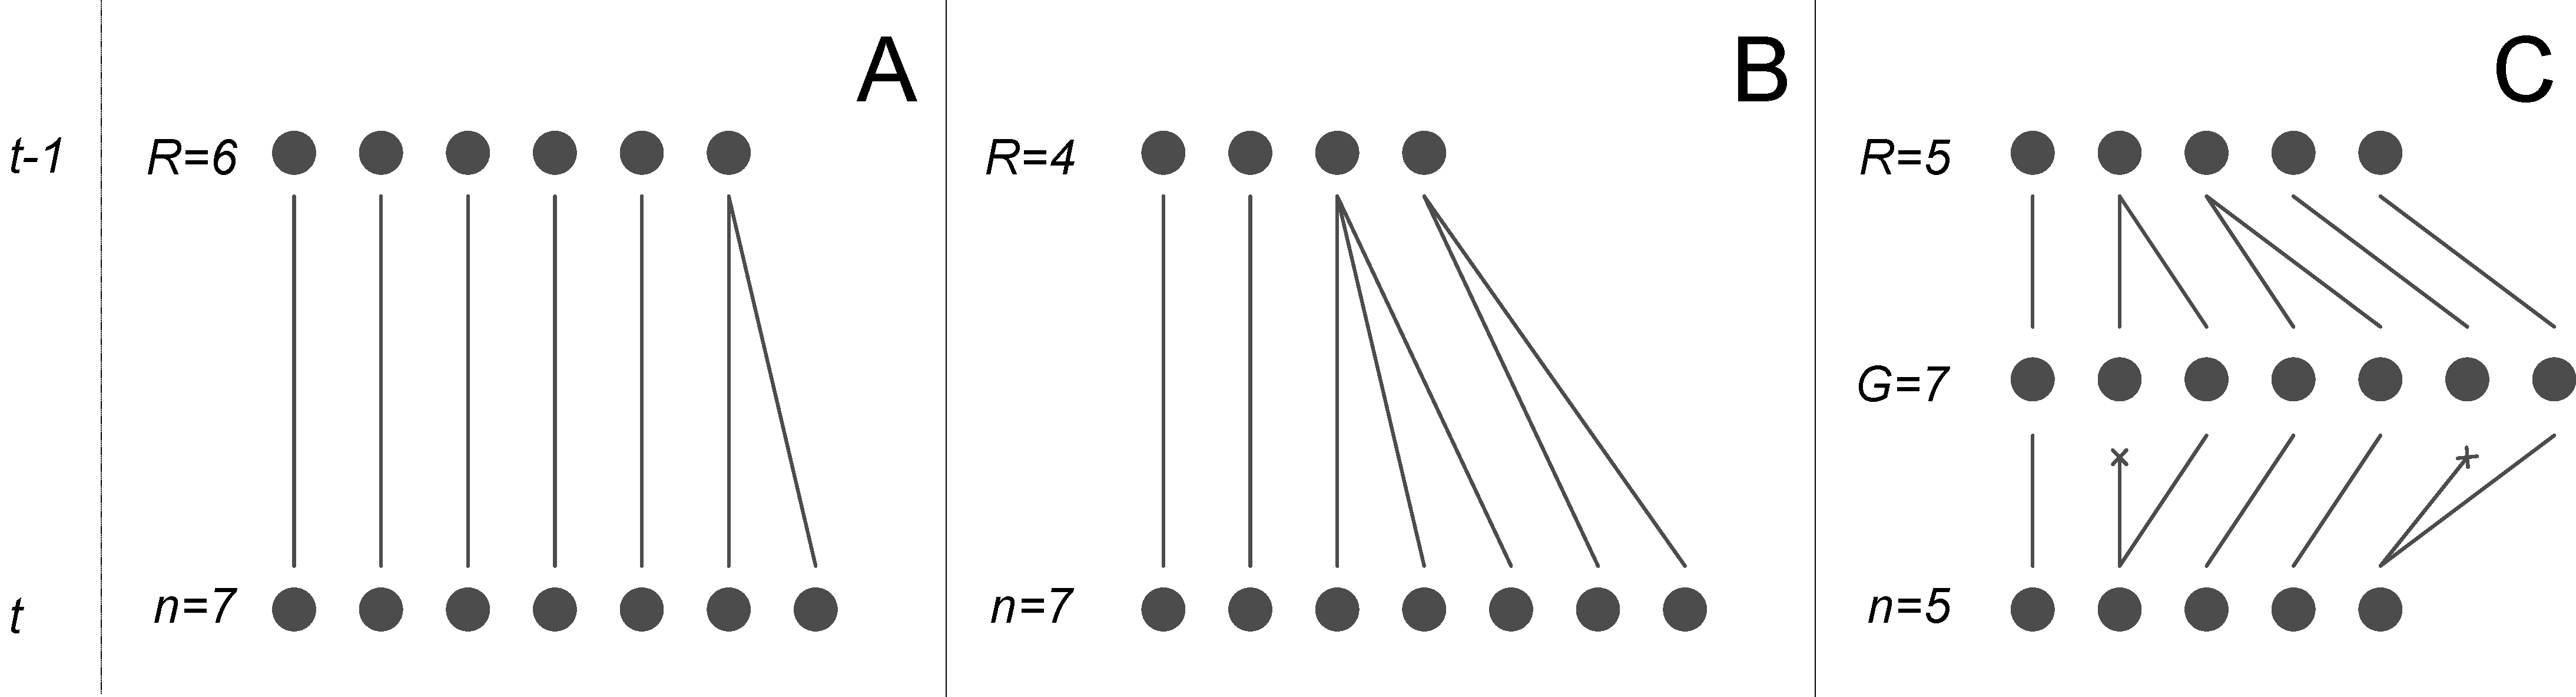
\includegraphics[width=1.0\textwidth]{fig/schematic.pdf}
  \caption{\label{fig:schematic} Realizations of sampling parental lineages under neutrality (A) and
    under selection (B,C). The top and bottom rows respectively represent the $n_p$ parents and $n_o$ offspring, 
    with the middle row in panel C representing the $n_g$ drawn gametes.
    Filled circles indicate the $i_p$, $i_g$, or $i_o$ copies of the derived allele. A line connecting
    two circles represents a successful draw, a broken line - a selective death triggering a redraw.
    %\textbf{A)} Under neutrality, possible coalescent events imply that number of parental lineages
    %$n_p$ at time $t-1$ is less than or equal to $n_o$ offspring lineages at time $t$. \textbf{B)}
    %With selection, re-sampling events are also possible, thus the possibility that $n_p \ge n_o$.
    %The net number of selection minus the coalescent events will indicate if the equations close.
    %\textbf{C)} We can also consider the number of gametes ($n_g$) produced. If we posit that
    %production of gametes is neutral, and the passing of gametes to offspring is under the control
    %of selection, we can develop a more intuitive understanding of the interplay of the two forces.
    %The version of the model with counting gametes is used to derive asymptotic results. 
    }
\end{figure}

To express the allele-frequency spectrum $\afs{n_o}{t}(i_o)$ for $n_o$ offspring in terms of the
\textit{AFS} at time $t-1$, we can sum over $n_p$ and the number $i_p$ of distinct derived alleles among them:

%\begin{equation}
%\afs{n_o}{t}(i_o)=\sum_{n_p,i_p} P_{n_o}(i_o,i_p,n_p) = 
%                  \sum_{n_p,i_p} P_{n_o}(i_o|i_p,n_p) P_{n_o}(i_p,n_p),
%\end{equation}

\begin{equation}
\afs{n_o}{t}(i_o)=P_{n_o} (i_o) =\sum_{n_p,i_p} P_{n_o}(i_o,i_p,n_p),
\end{equation}

where the subscript $n_o$ indicates dependence on parameter $n_o$. To obtain a recursion on the
\textit{AFS}, we note that the order in which we draw new parental lineages in the Wright-Fisher
model is random. In other words, we could draw a random permutation of the parental population, and
select parents in order from this permutation. We will separate properties of this permutation,
which depend only on parental \textit{AFS}s, from properties of Wright-Fisher sampling. Concretely,
the event $(i_p,n_p)$ can be expressed as the intersection of two events, $\mathcal{C}_{n_p}(i_p)$
and $\mathcal{S}_{n_p}$. Event $\mathcal{C}_{n_p}(i_p)$ specifies that the first $n_p$ parental
lineages from the random permutation carry $i_p$ derived alleles (that is,
$P(\mathcal{C}_{n_p}(i_p)) =\afs{n_p}{t} (i_p)$). Event $\mathcal{S}_{n_p}$ requires that the
Wright-Fisher drawing process stops after exactly $n_p$ parental lineages have been drawn.

\begin{equation}
\begin{split}
\afs{n_o}{t}(i_o)&= \sum_{n_p,i_p} P_{n_o}(i_o, \mathcal{S}_{n_p}, \mathcal{C}(i_p,n_p) )\\
&=   \sum_{n_p,i_p} P_{n_o}(i_o, \mathcal{S}_{n_p}| \mathcal{C}(i_p,n_p) ) P(\mathcal{C}(i_p,n_p))\\
&=   \sum_{n_p,i_p} P_{n_o}(i_o, \mathcal{S}_{n_p}| \mathcal{C}(i_p,n_p) )  \afs{n_p}{t-1}(i_p)\\
&\equiv  \sum_{n_p,i_p}  \mathbf{T}_{n_p,n_o}     \afs{n_p}{t-1}(i_p).
\end{split}
\label{eq:recur}
\end{equation}

where the $\mathbf{T}_{n_p,n_o}$ can be thought of as $(n_o+1) \times (n_p+1)$ matrices whose row
and column indices correspond to the number of derived alleles in the offspring and contributing
parental lineages, respectively.

Under neutral evolution, only terms with $n_p\leq n_o$ are nonzero. The corresponding \textit{AFS}
can all be obtained by downsampling from $\afs{n_o}{t-1}$ (\textit{i.e.}, $\afs{n_p}{t-1} =
\mathbf{H}_{n_p,n_o} \afs{n_o}{t-1}$ for hypergeometric projection matrix $\mathbf{H}_{n_p,n_o}$ if
$n_p\leq n_o$), and Equation \eqref{eq:recur} provides a closed form recursion for $\Phi_{n_o}$.
This property was used in \cite{JouganousEtAl2017} to efficiently compute distributions of allele
frequencies under neutrality and for small sample sizes.

Under selection, $n_{p}$ may be larger than $n_o$, leading to a set of $N$ coupled equations that is
typically too large to solve numerically (in the diffusion limit, the number of coupled equations is
infinite). But if the number of drift events is typically larger than the number of selective
deaths, as happens in large sample sizes, the coupling is weak and we can restore approximate
closure by truncating Eq. \eqref{eq:recur}:

\begin{equation}
\begin{split}
  \afs{n_o}{t}(i_o)
  &\simeq \sum_{n_p=1}^{n_{o}} \mathbf{T}_{n_p,n_o}                      \afs{n_p}{t-1}\\
  &=      \sum_{n_p=1}^{n_{o}} \mathbf{T}_{n_p,n_o} \mathbf{H}_{n_p,n_o} \afs{n_o}{t-1}\\
  &\equiv \mathbf{Q}_{n_o}                                               \afs{n_o}{t-1}\\
\end{split}
\label{eq:truncated}
\end{equation}

A jackknife approximation \cite{Gravel2016} can be used to simulate the drawing of a small number of
additional lineages and improve upon this closure approximation
($\afs{n_p}{t} \simeq J_{n_p,n_o} \afs{n_o}{t}$ with $n_p>n_o$). \cite{JouganousEtAl2017} used this
to derive approximate recursion equations under weak selection. We will show below that closure is
asymptotically maintained for large sample sizes even without requiring a jackknife approximation.

Our first goal is to obtain an explicit recursion for the matrices in \eqref{eq:recur}. To do so, we
will need to account for multiple coalescent events, which will require some careful bookkeeping.

\section{Transition probability matrices}
\label{sec:trans-mat}

\subsection{Constructing the transition matrix}
\label{subsec:trans-mat}

Even though $\mathbf{T}_{n_p,n_o}$ is a simple combinatorial probability describing a single
generation in the Wright-Fisher model, we were unable to compute an analytical expression for it,
while allowing for multiple coalescences and multiple selective events. However, we can obtain
fairly simple recursions by noting that properties of a sample of size $n_o$ are related to
properties of samples size $n_o-1.$ Similar recursions on sample size were used for describing large
sample size effects without selection in \citep{BhaskarEtAl2014}. In this section, we provide some
intuition for the recursion equation, and a more detailed derivation is provided in methods.

This recursion exists because the Wright-Fisher sampling can be performed one offspring at a time,
and even one draw at a time. The number of derived and ancestral alleles among the parents and the
offspring after a draw is related in a simple manner to the number of derived and ancestral alleles
prior to this draw. The transition from $n_o-1$ to $n_o$ successfully drawn offspring can involve an
arbitrary number $r$ of selective deaths. 

To keep track of this, we define $\mathbf{T}_{r}\Coalc{i_p}{n_p}{i_o}{n_o}$ as the probability
$P_{n_o}(\mathbf{Q}(i_o,r) | i_p, n_p)$ of the event $\mathbf{Q}(i_o,r)$ that exactly $i_o$ of the
first $n_o$ successfully drawn offspring are derived, and that the following $r$ draws are selective
deaths - Figure \ref{fig:rec-selection-dynamic-fail}. This bracket notation is convenient to keep track of
the number of relevant parental lineages (at the top) and offspring lineages (at the bottom), at the
cost of obscuring their different probabilistic role.
  
The recursion over $r$ in $\mathbf{T}_{r}\Coalc{i_p}{n_p}{i_o}{n_o}$ is shown at the bottom of
Figure \ref{fig:rec-selection-dynamic-fail}. To obtain $r$ selective deaths, we must first have
obtained $r-1$ selective deaths, followed by a selective death. We simply keep track of whether the
last failure was from a previously drawn lineage (case \textit{rD}), in which case the number of
parental lineages is unchanged, or of a new lineage (case \textit{rC}), in which case $n_p$ and
$i_p$ increased by one in the last draw.
 
Thus we can obtain $\mathbf{T}_{r}\Coalc{i_p}{n_p}{i_o}{n_o}$ from
$\mathbf{T}_{r-1}\Coalc{i_p-1}{n_p-1}{i_o}{n_o}$ and $\mathbf{T}_{r-1}\Coalc{i_p}{n_p}{i_o}{n_o},$
and recursively back to terms of the form $\mathbf{T}_{0}\Coalc{\cdot}{\cdot}{i_o}{n_o}$.
  
To progress further, we must express $\mathbf{T}_{0}\Coalc{\cdot}{\cdot}{i_o}{n_o}$ in terms of
$\mathbf{T}_{r}\Coalc{\cdot}{\cdot}{\cdot}{n_o-1}$, that is, we want to condition on the last
successful draws. This last successful draw can be a previously sampled parental lineage (or not),
and can be derived (or not) giving rise to the four cases shown on Figure
\ref{fig:rec-selection-dynamic-fail}.
  
Combining these two recursions, and using caching to avoid re-computing previously computed values,
we can systematically compute all the terms in Equation \ref{fig:rec-selection-dynamic-fail}.

Unfortunately, the number of rejected lineages can be infinite in the Wright-Fisher process.
However, the probability of having multiple selective deaths for a single successful draw decreases
rapidly as $s^r.$ We therefore modify the Wright-Fisher model such that at most $r_{max}$ failed
draws \emph{per offpsring} are allowed, after which the next draw is immune to selection. Given
$s<1$, we can easily pick $r_{max}$ to ensure excellent convergence. We found that $r_{max}=4$, was
amply sufficient to consider strong negative selection up to $Ns=50$.

\begin{figure}
  \centering
  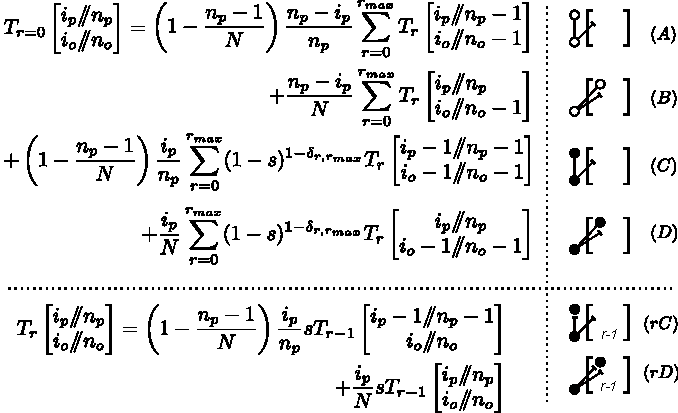
\includegraphics[width=0.9\textwidth]{fig/recurrence-selection-dynamic-failures-annotated.pdf}

  \caption{Recursion construct for transition probability with selection, accounting for multiple
    kinds of coalescent events. The right hand panel represents summands on the left graphically.
    Filled and empty circles represent derived and ancestral alleles. Solid and broken lines are
    successful lineage draws and re-draws due to selection. Double lines represent potentially
    multiple draws. Square brackets represent events in a smaller sample size ($n_o-1$). Summands
    (\textit{A-D}) are successful draws where the last lineage is ancestral (\textit{A,B}) or
    derived (\textit{C,D}). Note that these terms depend on the probability that there were between
    $0$ to $r_{max}$ selective events in sample size $n_o-1$. Terms \textit{rC} and \textit{rD}
    represent the probability that last selection re-draw was due to a lineage from outside
    (\textit{rC}) or within (\textit{rD}) the sample. See table \ref{tab:symbols} for notation used.
  }

  \label{fig:rec-selection-dynamic-fail}
\end{figure}
 
% Using a dynamic programming algorithm, we implement the construction of the exact neutral transition
% matrices $\mathbf{T}$ in $O(n^3)$ operations \sgcomment{We never talked about the neutral recursion, did we?
% Should we?}.
%  The set of selection transition probability matrices $\mathbf{T}$ requires $O(n^4+r_{max})$ operations. 
%  \sgcomment{Surely the $r_{max}$ term depends on n?}

\subsection{Calculation of allele frequency spectra}
\label{subsec:afs}

Once the truncated matrix
$\mathbf{Q}_{n_o} = \sum_{n_p=1}^{n_{o}} \mathbf{T}_{n_p,n_o} \mathbf{H}_{n_p,n_o}$ is constructed,
it can be used to calculate the allele frequency spectrum. To validate the method, we first use the
equilibrium distribution where exact solutions are available \cite{Krukov2016}. In the infinite sites
model at equilibrium, for example, we can compute the equilibrium \textit{AFS} $\Phi$ in a finite
sample as a solution to a linear system:

\begin{equation}
  \label{eq:sfs-calc}
  \Phi = Q \Phi  + n \mu e_1
\end{equation}

where $\mu$ is the per-site mutation rate, and $e_1$ is the first column of the identity matrix of
size $n$. Figure \ref{fig:strong-selection} shows the comparison of the \textit{AFS} calculated from
Equation \eqref{eq:coal-recursion, eq:sfs-calc}, the diffusion approximation \cite[eq.
9.23]{Ewens2004}, and the calculation performed in \texttt{Moments} \citep{JouganousEtAl2017}.

Figure \ref{fig:strong-selection}A-C show that there is a disagreement between the exact
Wright-Fisher and the diffusion solutions for singletons and doubletons. This effect increases as in
large sample sizes, as $n \ra N$, and has been reported by \citep{BhaskarEtAl2014}. There is a also
a divergence at high frequency of the derived allele. The Wright-Fisher and the present model are
both absorbing at fixation of the derived allele, while the diffusion are not. 

Figure \ref{fig:strong-selection}D shows a comparison at strong negative $Ns=50$, with the
population size ($N=1000$), which is substantially larger than the sample size ($n=100$). There is a
small deviation between the approaches at large allele frequencies. If the sample size is the same
as the population size ($n=N=100$) (Fig. \ref{fig:strong-selection}D), the diffusion approximation
and \texttt{Moments} depart from the Wright-Fisher prediction. The approach presented in this work
(Fig. \ref{fig:rec-selection-dynamic-fail}) shows a better match to the Wright-Fisher model.

\begin{figure}
  \centering
  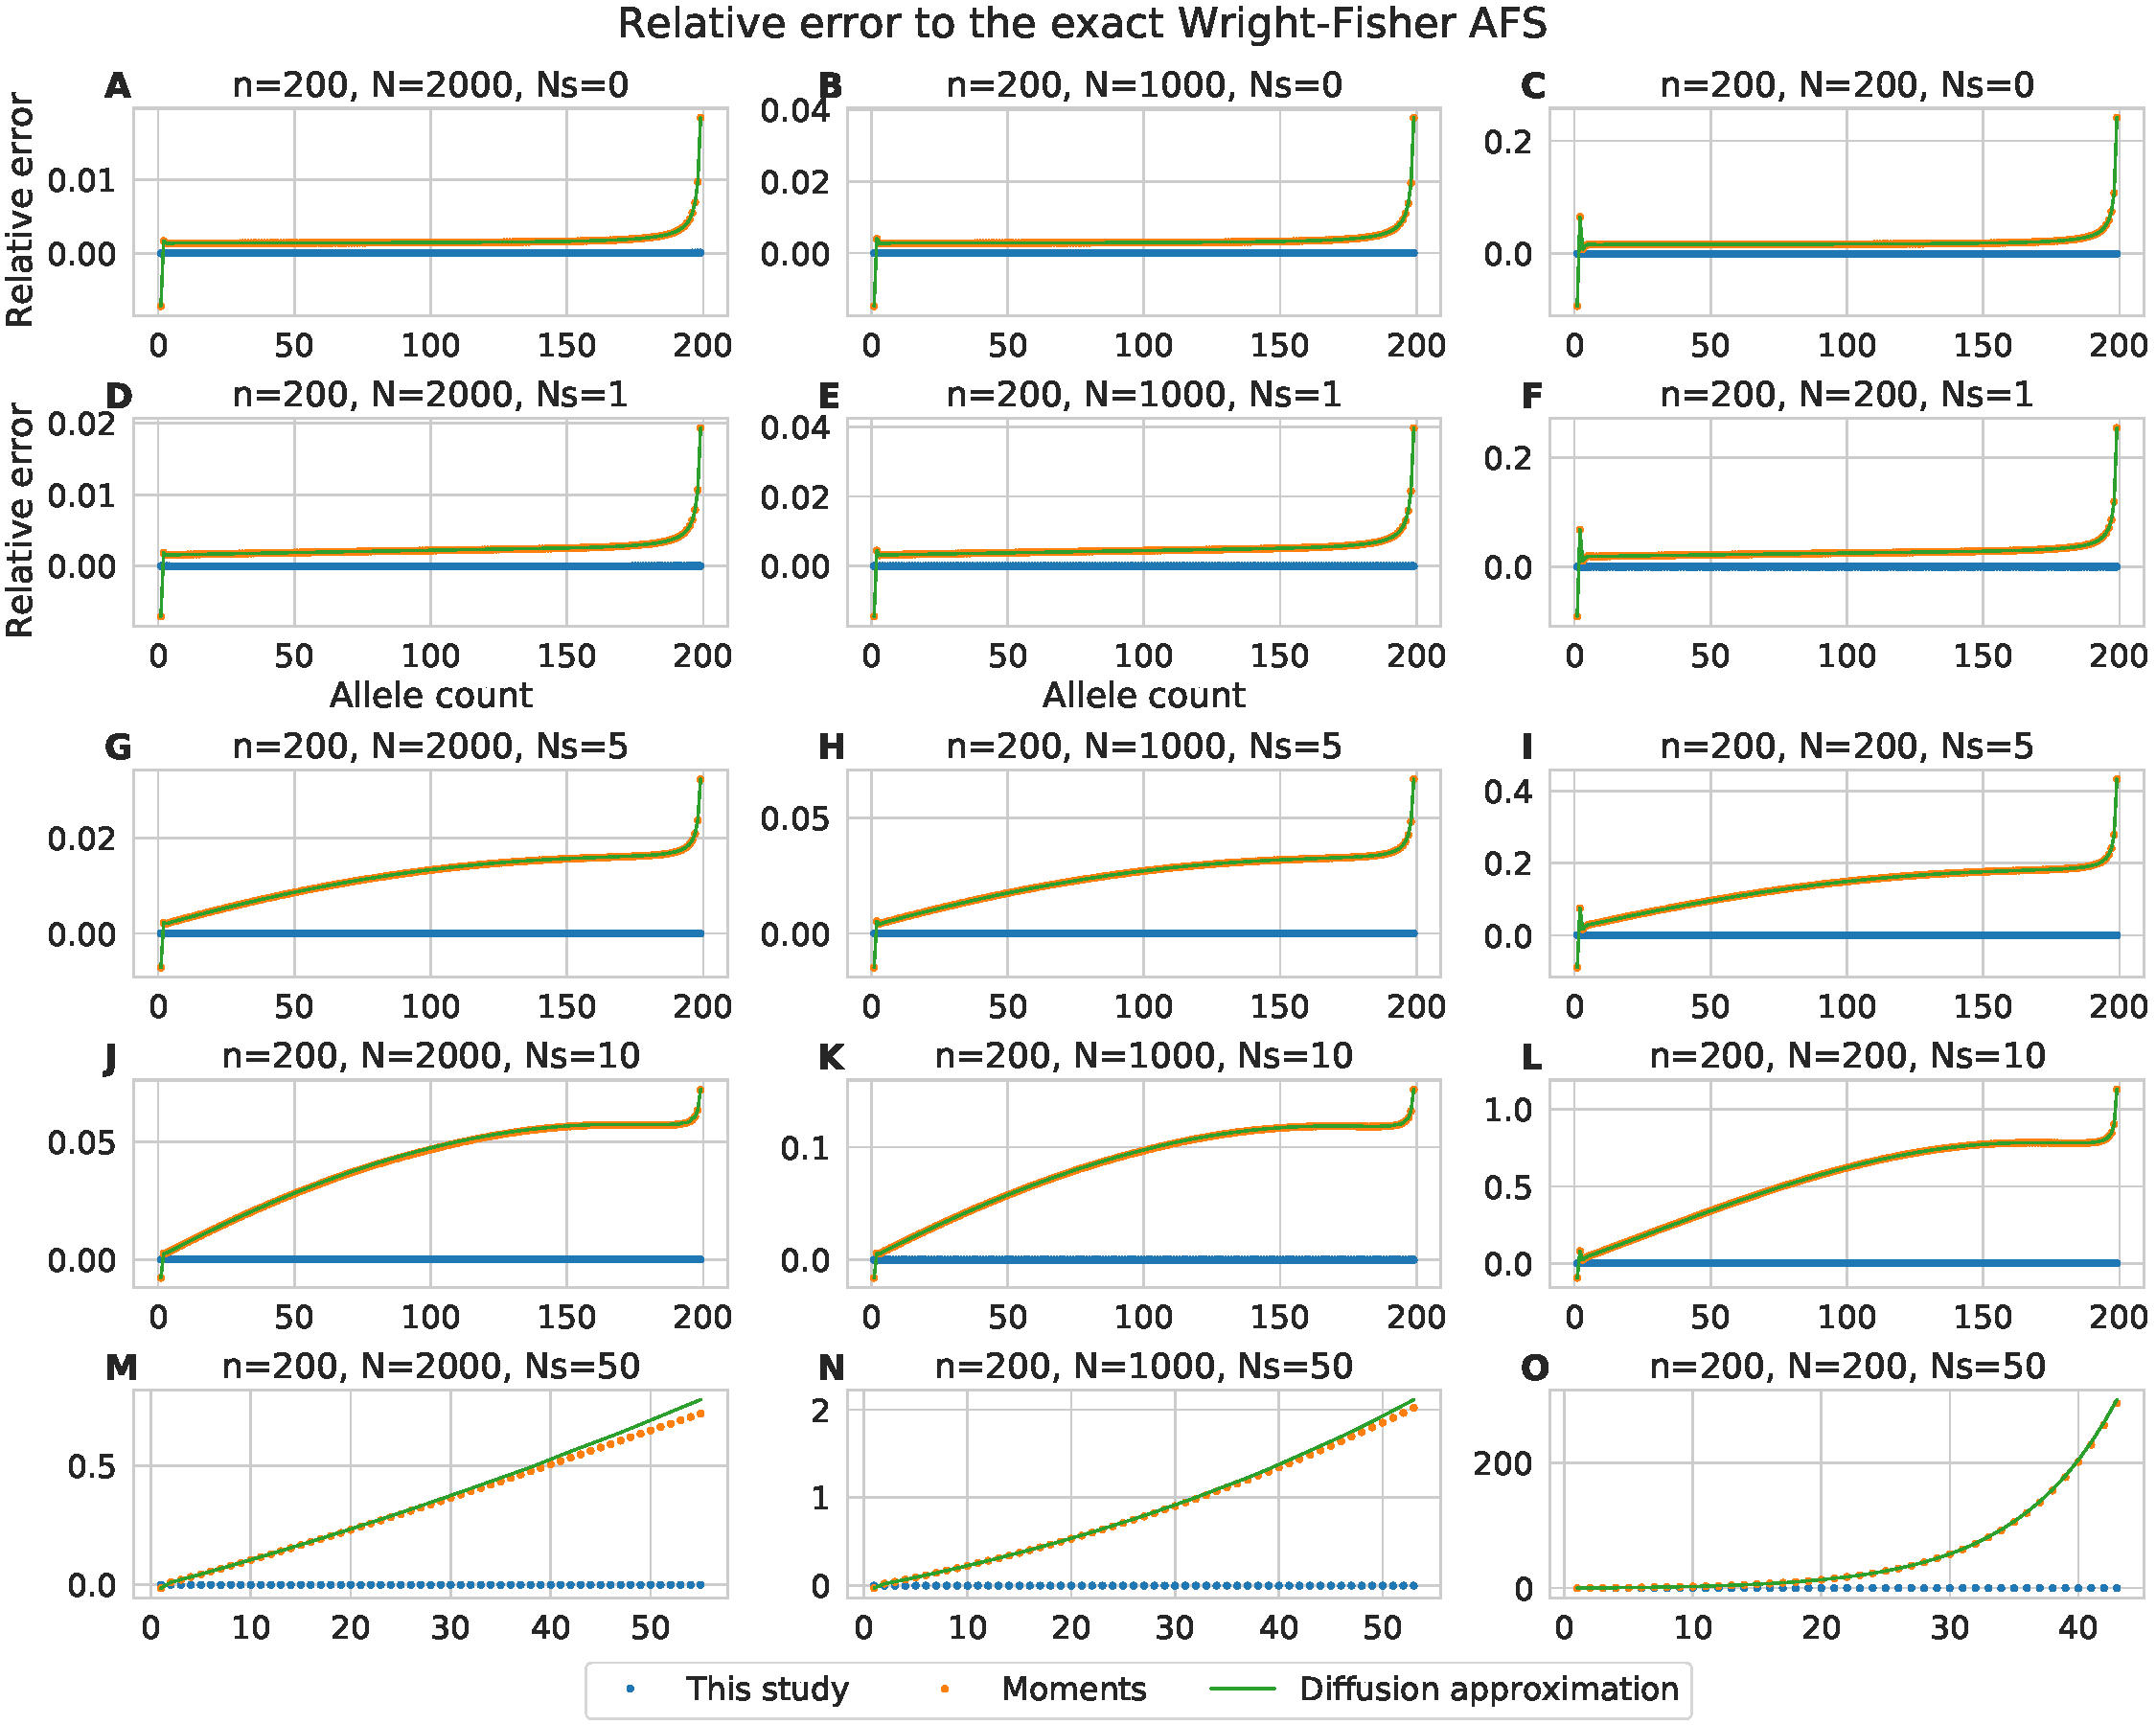
\includegraphics[width=0.7\textheight]{fig/strong_selection_six_panel.pdf}
  \caption{Normalized allele frequency spectra in a sample of size $n=100$, for neutral (Ns=0)
    (A,B,C), or highly deleterious alleles ($Ns=50$) (D,E,F). (A) shows the frequency spectrum in a
    sample from a large population ($N=1000$), (B) intermediate ($N=500$), and (C) small population
    ($N=100$). (D,E,F) same, for deleterious allele. The Y-axes are at different scales between the
    panels, to better indicate disagreement. The X-axes for panels (D,E,F) were truncated
    when the \textit{AFS} probability dropped below $10^{-12}$. }
  \label{fig:strong-selection}
\end{figure}

\subsection{Missing probability}
\label{subsec:missing}

Truncation in equation \ref{eq:truncated} means that if $n_p > n_o$, some lineages will be
unaccounted for. The transition matrix $\mathbf{Q}_{n_o}(i_p, i_o),$ in equation
\eqref{eq:truncated}, also has a probabilistic meaning:

The $(i_p,i_o)$th element of matrix $Q_{n_o}$ is the probability
 $P_{n_o}(i_o, \mathcal{S'}_{n_p}| \mathcal{C'}_{n_p}(i_p))$ that we observe $i_o$ derived alleles in
 a sample of size $n_o$ and that we draw \emph{at most} $n_o$ distinct parental lineages (event
 $\mathcal{S'}_{n_o}$), given event $\mathcal{C'}_{n_p}(i_p)$ that $i_p$ that $i_p$ of the first
 $n_p$ parental alleles are derived.

By summing $\sum_{i_o} \mathbf{Q}_{n_o}{i_p, i_o},$ we therefore get the proportion of draws that
were not truncated. $1-\sum_{i_o} \mathbf{Q}_{n_o}{i_p, i_o}$ is therefore the fraction of
unaccounted-for draws due to truncation, given $i_p$ derived among the first $n_o$ parental
alleles. Since only derived lineages experience selection, the largest number of resampling events,
and therefore the largest number of unaccounted lineages, occurs when all alleles are derived,
$i_o = n_o$.

Figure \ref{fig:apx:missing} shows this probability under this worst-case scenario. The probability
of missing lineages first increases with increasing sample size, as the number of draws that can
result in selective deaths increases. However, the number of drift events eventually overtakes the
number of selective events, and the probability that we need additional lineages decreases rapidly
with sample sizes.


\subsection{Distribution of number of contributing lineages}
\label{subsec:distribution}

For a given sample size, the probability that $n_p$ parents have contributed is:

\begin{align}
  \label{eq:conditional}
  P(n_p | n_o) = \sum_{n_g} P(n_p | n_g,n_o)P(n_g | n_o) = \sum_{n_g} P(n_p | n_g)P(n_g | n_o) 
\end{align}
where $n_p$ and $n_g$ is the number of contributing parents and gametes, respectively (Fig.
\ref{fig:schematic}C). 

 parameterized by
probability of resampling - $s$, and the total number of trials before $n_o$ successes (\textit{i.e.}
$n_r+n_o$):

The distribution over the number of gametes, $n_g \geq n_o$, is given by the negative binomial,
parameterized by the number of successes -- where the probability of a successful draw is $1-s$.
Then the toual number of doaws required for $n_o$ successes is:

\begin{align}
  \label{eq:neg-binomial-trials}
  P(n_g|n_o) = \binom{n_g-1}{n_o-1}(1-xs)^{n_o}(xs)^{n_g-n_o},
\end{align}
where $x_p$ is the proportion of derived alleles in the parental generation.

Given $n_g$, the number of parental lineages follows the modified occupancy (also known as
Arfwedson) distribution \citep{Wakeley2009,ONeill2019,JohnsonEtAl2005}:

\begin{align}
  \label{eq:occupancy}
  P(n_p|n_g) = \frac{S_2(n_g,n_p) N!}{(N-n_p)! N^{n_g}}
\end{align}
where $S_2(n_g,n_p)$ is a Stirling number of the second kind, which is the number of ways to
partition $n_g$ gametes into $n_p$ parents (see \cite{JohnsonEtAl2005} section 10.4 for a thorough
treatment). %Note that the under drift, the number of parents will be smaller or equal to the number
%of gametes $n_p \le n_g$.


Combining the two distributions together through Eq. \ref{eq:conditional}, we get:

\begin{align}
  \label{eq:lineages-in-past}
   Pr(n_p|n_o) = \sum_{n_g=1}^{\infty} \frac{S_2(n_g,n_p) N!}{(N-n_p)! N^{n_g}} \binom{n_g-1}{n_o-1}(1-x_ps)^{n_o}(x_ps)^{n_g-n_o}
\end{align}

This distribution does not appear to have a simple analytical form. However, it can be computed
efficiently using methods presented in \citep{ONeill2019}. Figure \ref{fig:combined}A (dots) shows
the distribution of the number of contributing parental lineages for several selection coefficients
for a sample, with $n_o=200$, $x_p=1$. In the absence of selection, the distribution has zero
probability above $n_o=200$, as no extra lineages can be sampled. As the strength of selection is
increased, we begin requiring larger numbers of lineages.

\begin{figure}
  \centering
  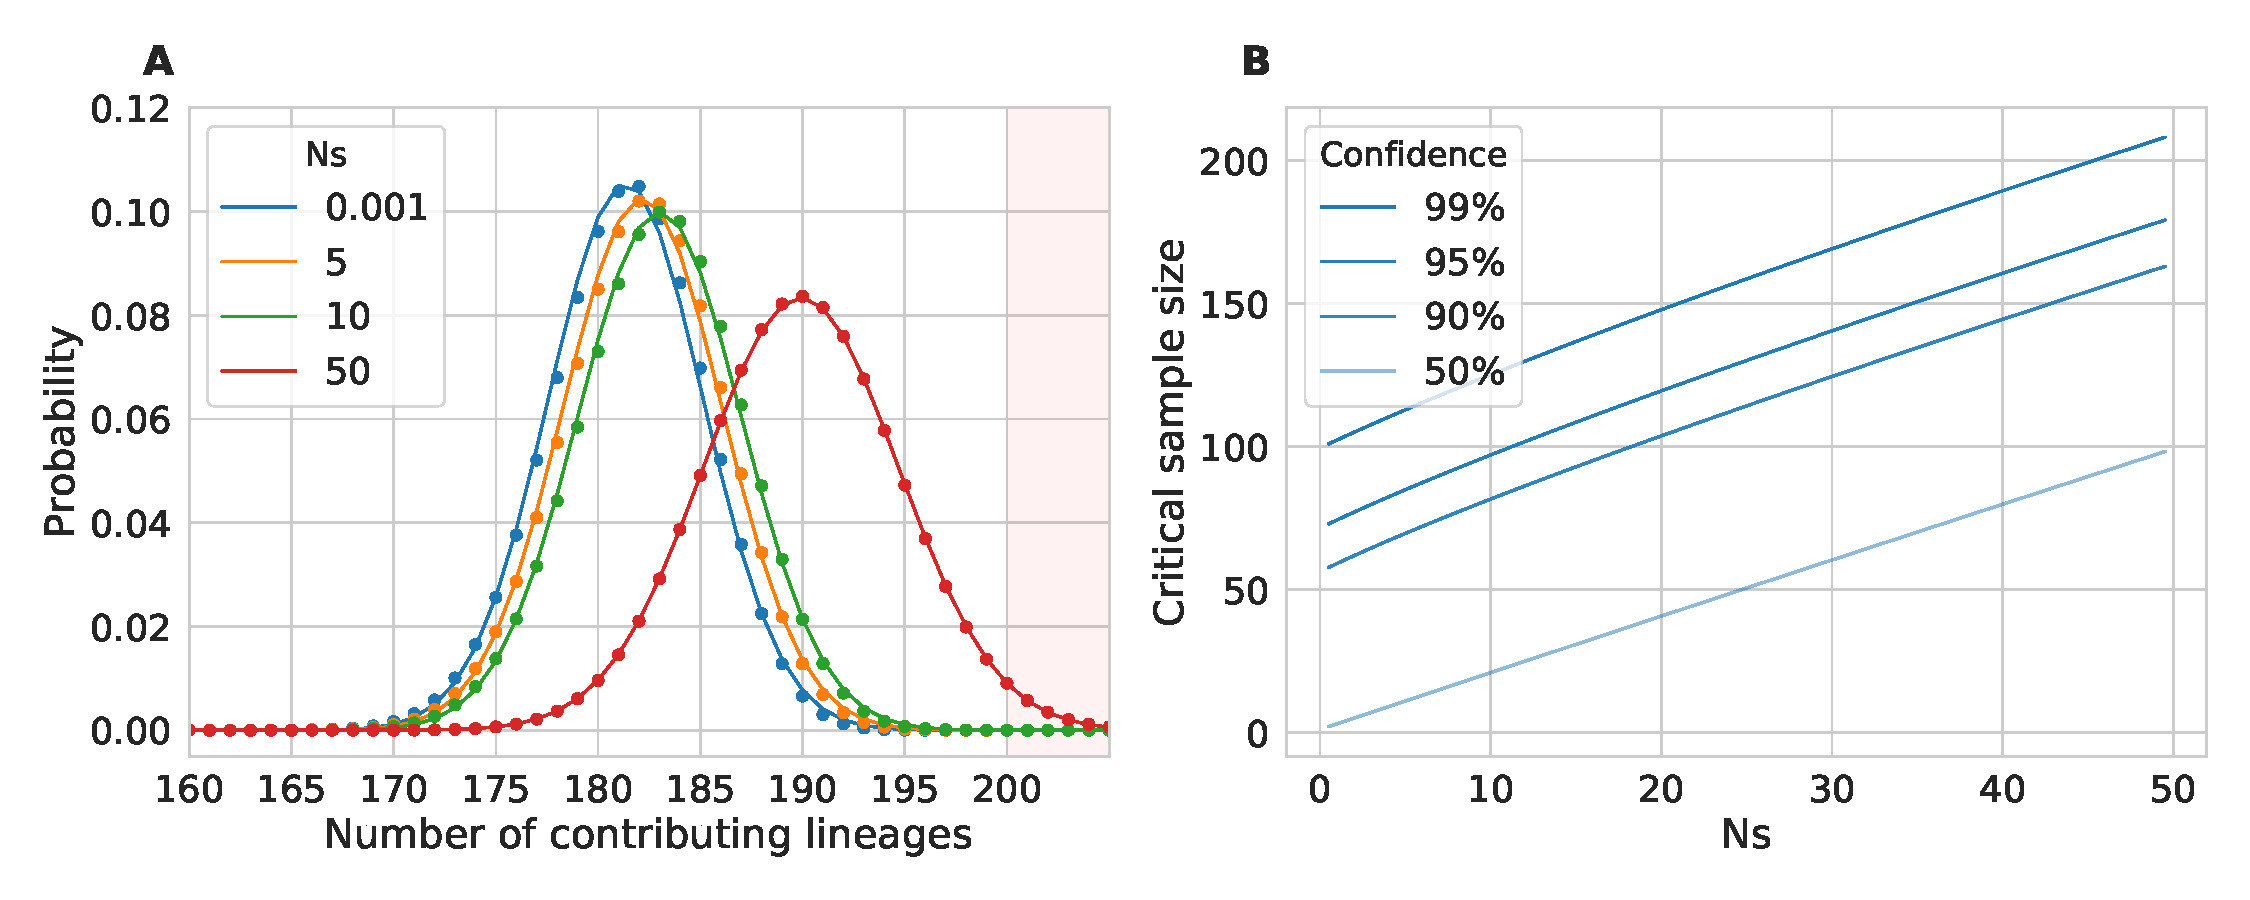
\includegraphics[width=\textwidth]{fig/combined.pdf}
  \caption{\textbf{A} The distribution of number of required lineages with $n_0=200$, $x_p=1$. Shaded
    red area shows missing probability - $n_p > n_o$. Points represent the exact probability one
    generation into the past (Eq. \ref{eq:lineages-in-past}), solid lines - Gaussian approximation
    (Eq. \ref{eq:gaussian}). \textbf{B} Sample size ($n_c$) as a fraction of population size ($N$)
    such that we have $99\%$ confidence that no lineages are missing. Derived from the Gaussian
    approximation. In both panels, $N=1000$.}
  \label{fig:combined}
\end{figure}

The distribution in Eq. \ref{eq:lineages-in-past} can be calculated effectively, but does not
provide a convenient way to answer the question - when are \textit{almost all} parental lineages
contained within the sample size $n_0$. For this, we will compute the expectation and variance 
of this distribution, and show that it is accurately described by a Gaussian approximation.

\section{Asymptotic closure properties}
\label{sec:asympt}

%We now want to estimate the sample size required to ensure that the system in Eq.
%\eqref{eq:truncated} remains almost closed. 


%In the following derivations, we are assuming that the derived allele is present in the parental
%generation at frequency $x = \frac{i_p}{n_p}$, instead of the discrete $i_p \dslash n_p$ in section
%\ref{subsec:trans-mat}, which simplifies the calculations. When looking for the upper bound on the
%number of rejected lineages, we take $x=1$, similar to section \ref{subsec:missing}.

%In addition, we now explicitly consider the number of gametes produced by the parents - as
%introduced in Fig. \ref{fig:schematic}C. The parental generation ($n_p$), produces a very large
%number of gametes, of which $n_g$ are randomly picked to contribute to the offspring. Each derived
%allele is then passed to one offspring with probability $1-s$, ancestral with probability $1$. 
%\sgcomment{This definition is not consistent with previous one}
%With
%probability $s$, picking a gamete fails, then a new contributing gamete is sampled. The number of
%coalescent events is $n_g - n_p$, and the number of selective deaths is $n_g - n_o$.

%\subsection{Mean number of contributing lineages}
%\label{sec:mean-contr}

Using the law of total expectation, we can write the expectation $E[n_p-n_o | n_o]$ as 
\begin{equation*}
  \begin{aligned}
    \label{eq:lineages-approx}
    E[n_p-n_o | n_o] &=        E[n_p | n_o]       - n_o \\
                     &=E_{n_g} E_{n_p}[n_p | n_g] - n_o.
  \end{aligned}
\end{equation*}
Assuming $x_p\equiv i_p/n_p=1$, the expectation over $n_p$ is simply given by the occupancy distribution \cite{Wakeley2009}.

\begin{equation*}
  \begin{aligned}
    \label{eq:lineages-derive}
    \hat{E}[n_p -n_o | n_o]
    & =   E_{n_g}\left[N\left[1-\left(1 - \frac{1}{N} \right)^{n_g} \right]\right]- n_o\\
    & =   N-N  E_{n_g}\left[\left(1 - \frac{1}{N} \right)^{n_g} \right] -n_o. 
  \end{aligned}
\end{equation*}

As mentioned above, the number of selective deaths, $n_g-n_o$ follows a negative binomial distribution.
 We can use the moment generating function of the negative binomial to compute the expectation for
constant $k$,

\begin{equation}
E_{n_g}[k^{n_g}] = k^{n_o}  \left(\frac{1-s}{1-sk}\right)^{n_o}.
\label{eq:identity}
\end{equation} 

Thus we can write 
\begin{align}
  \label{eq:lineages-exact}
  \hat{E}[n_p -n_o | n_o] &= N-N\left( 1 - \frac{1}{N} \right)^{n_o}\left( \frac{1-s}{1-s \left( 1 - \frac{1}{N} \right)}\right)^{n_o}-n_o.
\end{align}

Taking the terms of order $\frac{1}{N}$ gives,

\begin{equation*}
    \label{eq:lineages-approx}
    \hat{E}[n_p-n_o | n_o] \approx n_os - \frac{n_o (n_o-1) }{2N}. 
\end{equation*}

We thus have the usual interplay of selection and drift. Solving for $ \hat{E}[n_p -n_o | n_o]<0$
yields, to leading order,

\begin{equation}
  \label{eq:critical-sample}
  n_o^* \ge 2Ns.
\end{equation}

This gives us a simple and convenient expression for the critical sample size, where there are more
drift than selection events, on average. However, closure of the recursions requires not only that
drift occurs more often than selection on average, but almost always.

Our next step is to compute the variance $\operatorname{Var}[n_p-n_o | n_o].$ The detailed
calculations are provided in the appendix, and the result is:

\newcommand{\vara}[1]{\left(1-\frac{#1}{N}\right)}
\newcommand{\varb}[1]{\left(\frac{1-s}{1-s #1}\right)}

\begin{equation}
  \begin{aligned}
    \operatorname{Var}[n_p-n_o | n_o] &=
    N^2\left( \vara{1}^{2n_o}\varb{\vara{1}^2}^{n_o}-\vara{1}^{2n_o}\varb{\vara{1}}^{2n_o} \right) + \\
    &+ N(N-1)\vara{2}^{n_o}\varb{\vara{2}} + \vara{1}^{n_o}\varb{\vara{1}}^{n_o} - \\
    &- N\vara{1}^{2n_o} \varb{\varb{1}^{2}}^{n_o}
  \end{aligned}
\end{equation}

% Figure \ref{fig:critical-sample-size} shows the critical sample size for several selection
% coefficients, assuming the entirety of the sample is derived ($x=1$) in a population of $N=1,000$.
% The $Y$ axis shows the fraction of contributing parental lineages to the sample size,
% $\frac{n_p}{n_o}$. Above the horizontal line $\frac{n_p}{n_o} > 1$, selection dominates. Below,
% drift reduces the number of used lineages. The intercept of the line with $\frac{n_p}{n_o} = 1$ is
% the critical sample size, which is well-approximated by $2Nsx$.

\subsection{Gaussian approximation}

%We can construct a Gaussian approximation to the distribution of the number of contributing lineages.
%This approximation will allow us to calculate sample size where, for example, the number of
%contributing lineages is smaller that the sample size $95\%$ of the time, instead of $50\%$, as
%given by $n_o^*$ in equation \eqref{eq:critical-sample}.

% A Gaussian with mean and variance caluclated above provides an excellent approximation to equation
% \eqref{}. This is not unexpected, since both the number of selective events and the number of drift
% events are well approximated by normal distributions: The occupancy distribution is approximated by
% the Gaussian distribution when $n_o \ll N$ \citep{ONeill2019}. Likewise, can the number of failures
% ($n_r$) before a given number of successes (negative binomial) \sgcomment{reference?}. In the case
% of large sample size, as required by the approximation of the occupancy by the Gaussian, we can
% approximate the total number of contributing lineages as the sum of lineages
% \sgcomment{??}contributed by the two distributions. Specifically, we require that the number of
% coalescent events is large, such that the occupancy distribution can be approximated well by the
% Gaussian: $\frac{{n_o^*}^2}{2N} \ge 10$. \sgcomment{I am confused by this paragraph.}

We use a Gaussian distribution with the mean and variance defined above to approximate the
distribution of the required parental lineages. Figure \ref{fig:combined}A shows the exact
distribution as dots, and the Gaussian approximation as solid lines. In this parameter regime, we
have good agreement between the two computation methods.


For the approximation to work well, we require that the sample size is sufficiently large with
respect to the population size, namely that $\lambda \equiv \frac{{n_o^*}^2}{2N} \ge 10$, similar to
the conditions for the Poisson distribution to be approximated with the Gaussian.

We can then numerically compute the quantiles of the Gaussian distribution to find a sample size
where we are, for example, $99\%$ confident that there will be no missing lineages. Figure
\ref{fig:combined}B shows this as sample size ($n_o$) over the population size ($N_e$), for
different population sizes. The dashed lines indicate where the Gaussian approximation may be
invalid: $\lambda \le 10$.

Figure \ref{fig:apx:critical-fraction} shows the critical sample size as a fraction of the total
population size.

\subsection
{Integrating over several generations} 

If the sample size is large enough that $E[n_p-n_o]<0$, but not large enough that
$P(n_p>n_o) \ll 1,$ we can improve the truncation by integrating over more than one generation.
Lineages gained by selective death at one generation can be compensated for by genetic drift at
another generation. Informally, the expected change $E[n_g-n_o]$ in the number $n_g$ of lineages in
the grandparent generation relative to $n_o,$ and the variance $\operatorname{Var}(n_g-n_o)$ will be
roughly double those over a single generation. Thus the z-score determining the amount of
unnaccounted-for lineages in the normal approximation,
$z= E[n_g-n_o] / \sqrt{\operatorname{Var}(n_g-n_o)}$ will increase roughly by a factor $\sqrt{2}$.

Such transition matrices can also be computed iteratively. If $n_{p'}$ is the number of contributing
lineages in the grandparental generation, and $i_{p'}$ is the number of derived alleles among those,
and we define $P(i_o, n_{p'} | q(i_{p'}, n_{p'}))$, as above, as the probability of drawing $i$
derived alleles and using exactly $n_{p'}$ grandparental alleles given the event $q(i_{p'}, n_{p'})$
that $i_{p'}$ of the first $n_{p'}$ grandparental alleles are derived \sgcomment{We would need to
  reconcile the notation here with the previous one}, we can condition on the number of contributing
parental alleles $n_p$ and the number of derived alleles $i_p$ among them in the parental
generation: \sgcomment{define $S'$}
 
 \begin{equation}
 \begin{split}
 P(i_o, \mathcal{S}'_{n_p'} | \mathcal{C}'(i_{p'}, n_{p'})) & = \sum_{i_p,n_p} P(i_o, \mathcal{S}'_{n_p'} ; \mathcal{C}(i_p,n_p), \mathcal{S}_{n_p} | \mathcal{C}'(i_{p'}, n_{p'}))\\
 &= \sum_{i_p,n_p}  P(i_o, \mathcal{S}'_{n_p'} | \mathcal{C}(i_p,n_p), \mathcal{S}_{n_p} ; \mathcal{C}'(i_{p'}, n_{p'})) P\mathcal{C}(i_p,n_p), \mathcal{S}_{n_p} | \mathcal{C}'(i_{p'}, n_{p'}) \\
 &=  \sum_{i_p,n_p}  P(i_o, \mathcal{S}'_{n_p'} | \mathcal{C}(i_p,n_p), \mathcal{S}_{n_p})) P\mathcal{C}(i_p,n_p), \mathcal{S}_{n_p} | \mathcal{C}'(i_{p'}, n_{p'}) \\
 &=   \sum_{n_p} T_{n_p,n_o} T_{n_{p'}, n_p},
 \end{split}
\end{equation}
 %&= \sum_{i_p,n_p} P(i_o, n_p,  r(i_p,n_p); n_{p'}  | q(i_{p'}, n_{p'}))\\
 %&= \sum_{i_p,n_p} P(i_o, n_p|   r(i_p,n_p); n_{p'}  ; q(i_{p'}, n_{p'}))  P(r(i_p,n_p); n_{p'}  | q(i_{p'}, n_{p'}))\\
 %&= \sum_{i_p,n_p} P(i_o, n_p |   r(i_p,n_p))  P( r(i_p,n_p); n_{p'}  | q(i_{p'}, n_{p'}))\\
 %&= \sum_{i_p,n_p} P(i_o, n_p |   r(i_p,n_p))  P( r(i_p,n_p); n_{p'}  | q(i_{p'}, n_{p'}))
where the sum over $i_p$ is part of the product of the transition matrices $T$. 
Since each matrix product takes \sgcomment{scaling of practical matrix product algos}, and there or $o(n)$
such products, the computation of this matrix takes at most \sgcomment{...}.



\section{Conclusion}
\label{sec:conclusion}

Classically, the coalescent considers models in the absence of natural selection. Since selection
can increase the number of contributing lineages back in time, the coalescent can no longer be
represented by trees, but instead acquires a graph structure. The ancestral selection graphs
\citep{KroneNeuhauser1997} deal with this in the limit of large population size ($N$).

The large population size approximation implies that the sample size $n$ is much smaller than the
whole population ($n \ll N$), so it is unlikely that more than one coalescent event will happen per
generation. However, recent work \citep{BhaskarEtAl2014,NelsonEtAl2019} pointed out that this
assumption is unreasonable with sample sizes pertinent to modern experiments. As a results, models
that consider multiple coalescent events per generation are gaining increased relevance in the
field \citep{FlemmingtonVoit}.

In this work we show that increasing the sample size has another unexpected consequence. As sample
size increases, the larger number of lineages needed due to selection can be masked by coalescent
events. In this sense, the large sample size rescues the model from effect of selection. This means
that recursion equations needed to calculate sample properties are asymptotically closed with large
population size.

At first approximation, $n_o^*=2Nsx$ is a critical sample size, where the decrease of lineages due to
coalescent back in time out-competes the increase due to selection (eq. \eqref{eq:critical-sample}).
Further, we derive the full probability distribution for the number lineages needed with given
selection coefficient and sample size (eq. \eqref{eq:lineages-in-past}). Unfortunately, the
distribution does not have a closed form, so we derive a normal approximation to the number of
lineages that contribute to a sample (eq. \eqref{eq:normal-approximation}). The normal approximation
then allows us to get a quantile function that we use to find if the model preserves closure with
some confidence level.

This work has several implications. First, we can combine the model described here with the
jackknife approximation \citep{JouganousEtAl2017}. This will allow us to construct a more robust
inference framework that can account for large sample size and strong selection.

Further, the results here suggest that effect of weak selection may be detectable in studies with
large sample sizes. This may open up a way for new investigations of natural selection in population
genetics.

\bibliography{disco}

\section{Appendix}
\renewcommand{\thefigure}{S\arabic{figure}}
\setcounter{figure}{0}

\subsection{Missing lineages}

\begin{figure}
  \centering
  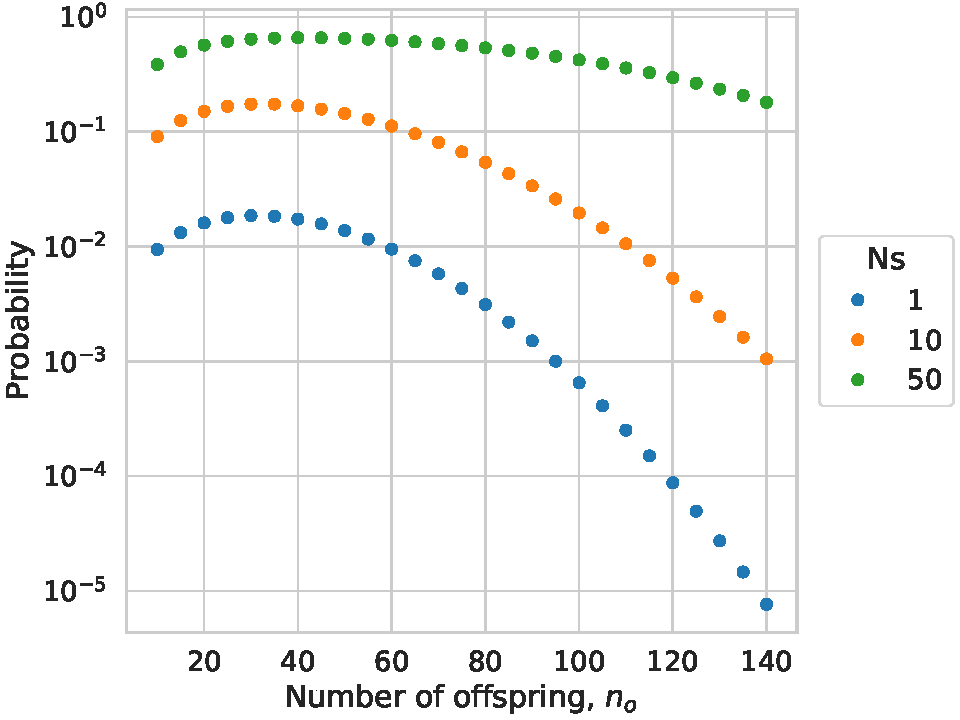
\includegraphics[width=\textwidth]{fig/missing.pdf}
  \caption{Probability that there are more contributing parents than offspring, $n_p > n_o$.
    Calculated as $1-\sum_{i_o} \mathbf{Q}_{n_o}{i_p, i_o}$, $N=1000$.}
  \label{fig:apx:missing}
\end{figure}

\subsection{Quantiles of the Gaussian approximation}

Figure \ref{fig:apx:critical-normal} shows the critical sample size for a given quantile of the normal
approximation, as a function of the population-scaled selection coefficient. The $50^{\text{th}}$
percentile corresponds to the mean calculated in equation \ref{eq:critical-sample} ($\approx 2Ns$).
If we want to ascertain that the distribution is closed with increased confidence, we require a
larger number of lineages. All curves assume $N=1000$.

\begin{figure}
  \centering
  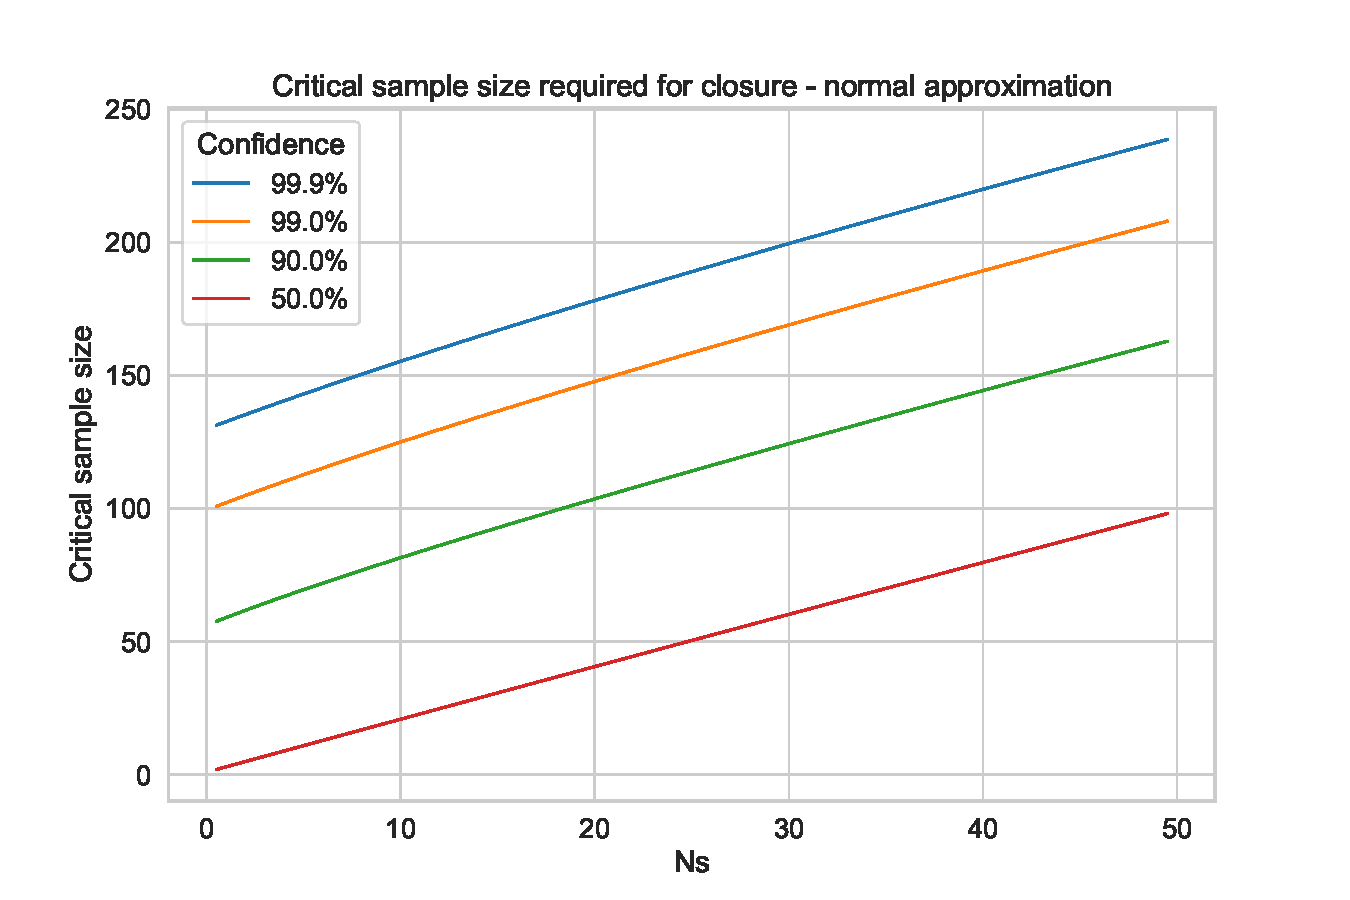
\includegraphics[width=\textwidth]{fig/critical_normal.pdf}
  \caption{Critical sample size that is required for a given closure confidence level. The $50^\text{th}$ percentile corresponds to the mean in the equation \eqref{eq:mean}. Note that the normal approximation is invalid for $Ns=0$, where the occupancy distribution should be used. All lines are calculated with $N_e=1000$.}
  \label{fig:apx:critical-fraction}
\end{figure}

\subsection{Variance of number of contributing lineages}
\label{subsec:apx:variance}

We can obtain the variance of the distribution $Pr(n_p | n_o)$ by using the law of total variance:

\begin{equation}
  \label{eq:apx:var}
\Var\left[n_p-n_o \right] = \Var_{n_g}\left[E\left[n_p-n_o | n_g \right]\right]+  E_{n_g}\left[Var\left[n_p-n_o | n_g \right]\right] 
\end{equation}

The expectation in the first term can be derived from the occupancy distribution and the identity
\ref{eq:identity}:

\begin{equation}
\begin{split}
\Var_{n_g}\left[E\left[n_p-n_o | n_g \right]\right] &= \Var_{n_g}\left[E\left[n_p| n_g \right]\right] \\
&= \Var_{n_g}\left[N\left(1-(1-\frac{1}{N})^{n_g} \right) \right] \\ 
&= N^2 \Var_{n_g}\left[(1-\frac{1}{N})^{n_g} \right] \\
&= N^2 \left( E_{n_g}\left[(1-\frac{1}{N})^{2n_g} \right] - E_{n_g}\left[(1-\frac{1}{N})^{n_g} \right]^2\right) \\
&= N^2 \left( \left(1-\frac{1}{N}\right)^{2n_o} \left(\frac{1-s}{1-s  \left(1-\frac{1}{N}\right)^2}\right)^{n_o} 
-   \left(1-\frac{1}{N}\right)^{2n_o} \left(\frac{1-s}{1-s  \left(1-\frac{1}{N}\right)}\right)^{2n_o} \right) \\
\end{split}
\end{equation}

The variance of the second term is the variance of the occupancy distribution \cite{}:

\begin{equation}
\begin{split}
E_{n_g}\left[Var\left[n_p-n_o | n_g \right]\right] & = E_{n_g}\left[N ((N - 1) (1 - 2/N)^{n_g} + (1 - 1/N)^{n_g} - N (1 - 1/N)^{2 n_g}) \right] \\
& = N (N-1)  \left(1-\frac{2}{N}\right)^{n_o} \left(\frac{1-s}{1-s  \left(1-\frac{2}{N}\right)}\right)^{n_o} +  \left(1-\frac{1}{N}\right)^{n_o} \left(\frac{1-s}{1-s  \left(1-\frac{1}{N}\right)}\right)^{n_o} \\
&-N  \left(1-\frac{1}{N}\right)^{2n_o} \left(\frac{1-s}{1-s  \left(1-\frac{1}{N}\right)^2}\right)^{n_o}. 
\end{split}
\end{equation}

The two terms can be summed together to provide an analytical expression for the variance of $n_p$. 

\subsection{Neutral case}

We want to construct the entries in the probability matrix
$P\left[ \Dfrac{\cdot}{n_o} \cond \Dfrac{\cdot}{n_p} \right]$ in terms transition probabilities in
smaller sample sizes. Under neutrality, the number of contributing parental lineages $n'_p$ (at
$t-1$) can not be larger than the number of offspring lineages $n_o$. Since $\mathbf{P}$ is square,
$max(n_p)=max(n_o)=n$. Thus, our aim is to express every entry of $\mathbf{P}$,
$P\left[ \Dfrac{\cdot}{n} \cond\Dfrac{\cdot}{n} \right]$, in terms of
$P\left[ \Dfrac{\cdot}{n-1} \cond \Dfrac{\cdot}{n-1} \right]$. Since we never require extra lineages
($n_p\le n_o$), the recurrence is closed.

To calculate the transition probabilities, we first condition on the state of the last parental
allele drawn, and then on the coalescent event that last offspring lineage participates in. The
recurrence is shown in figure \ref{fig:rec-neutral}. The panel on the right depicts the coalescent
event for each term. Empty circles represent ancestral alleles, filled circles -- derived. The
square box represents a sample of size $n-1$. The first three terms in the sum correspond to the
cases where the last parent that we drew was ancestral, last three -- derived.

\begin{figure}
  \centering
  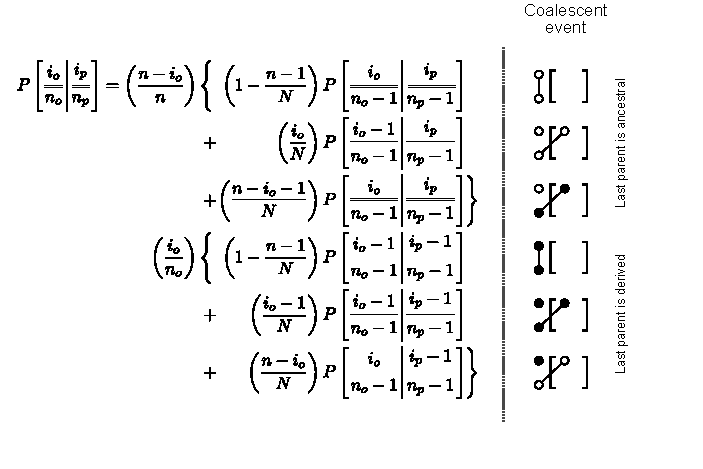
\includegraphics[width=0.9\textwidth]{fig/recurrence-neutral-annotated.pdf}
  \caption{Recurrence defining transition probabilities in a model without selection. Right panel
    shows coalescent events corresponding to each summand. Each transition probability is defined in
    terms of transition in a smaller sample size. First three terms are conditional on the last
    parent having an ancestral state, last three -- derived. Filled circles -- derived alleles;
    empty circles - ancestral alleles; square brackets -- sample of size $n-1$.}
  \label{fig:rec-neutral}
\end{figure}

When calculating a single entry in \ref{fig:rec-neutral}, the variables have the following ranges.
\begin{equation}
  \begin{aligned}
    n_p &= n \\
    i_p &\in [0, n] \\
    n_o &= n \\
    i_o &\in [0, n] \\
  \end{aligned}
\end{equation}

The recurrence is calculated while $n>1$, with the following base cases:
\begin{align*}
  P\left[ \Dfrac{1}{1} \cond \Dfrac{1}{1} \right] &= 1 \\
  P\left[ \Dfrac{0}{1} \cond \Dfrac{0}{1} \right] &= 1 \\
  P\left[ \Dfrac{0}{1} \cond \Dfrac{1}{1} \right] &= 0 \\
  P\left[ \Dfrac{1}{1} \cond \Dfrac{0}{1} \right] &= 0 \\
\end{align*}

\subsection{Selection case}

\ikcomment{I've changed the event $r$ to $c$ in the main text (to avoid the unlikely confusing for
  $r$, the number of failures). This will need to be propagated in here, too}.

Due to selective deaths, the number of lineages ($n_p$) that contribute to the current generation
can be larger than the number of offspring ($n_o$), and especially so with strong selection. Because
the number of sampling configurations can be large, we use dynamic programming to estimate
$\mathbf{P}_{n_p,n_o}$ by summing over the possibilities for the last successful draw. Using the
probability interpretation of the transition matrix,
$\mathbf{P}_{n_p,n_o}(i,j) = P(i, n_p | r(j, n_p)),$ the probability that we draw $i$ derived
offspring and exactly $n_p$ parental offspring given that $j$ of the first $n_p$ sampled parental
alleles are derived. The last successful draw event can be specified by the number
$t \in \{0,\infty\}$ of prior failed draws due to selection since the last successful draw, the
allele $a \in {A, D}$ selected, and the event $c$ of whether or not the sampled parental allele was
previously drawn $c\in \{True, False\}$. We also consider the event $s \in \{True, False\}$ of
whether the last draw was successful. Finally, let us define the event $E_{n_o,t}(i,n_p)$ that we
have drawn $i$ derived offspring among $n_o$ successful draws followed by $t$ failures, and that
this required exactly $n_p$ parental lineages.

\begin{equation}
\begin{split}
P(i, n_p | r(j, n_p)) = P(E_{n_0,0}(i,n_p)  | r(j, n_p)) &=  \sum_{a, c,t} P(a,c,t; E_{n_o,0}(i,n_p)  | r(j, n_p)) 
 \end{split}
\end{equation}

Let us consider the term $a=A$, $c=False$ \sgcomment{We could use a better notation here, eg using
  tikz. }

\begin{equation}
  \begin{split}
    P(a=A,c=False,t; E_{n_o,0}(i,n_p)  | r(j, n_p)) &= P(a=A, c=False, t,s=True; E_{n_o,t}(i,n_p-1) | r(j, n_p))\\
    &= P(a=A, c=False, t; E_{n_o,t}(i,n_p-1) | r(j, n_p))\\
    &=P(a=A, c=False, t ; E_{n_o,t}(i,n_p-1); r(j, n_p-1) | r(j, n_p))\\
    &=P(a=A, c=False, t ; E_{n_o,t}(i,n_p-1)| r(j, n_p-1)  r(j, n_p)) P(r(j, n_p-1) |  r(j, n_p))\\
    &=P(c=False, t;  E_{n_o,t}(i,n_p-1) | r(j, n_p-1)  r(j, n_p)) \frac{n_p-j}{n_p}\\
    &=P(c=False | t;  E_{n_o,t}(i,n_p-1) | r(j, n_p-1)  r(j, n_p)) P(t;  E_{n_o,t}(i,n_p-1) | r(j, n_p-1)  r(j, n_p)) \frac{n_p-j}{n_p}\\
    &=\left(1-\frac{n_p-1}{N}\right) P(t;  E_{n_o,t}(i,n_p-1) | r(j, n_p-1)  r(j, n_p)) \frac{n_p-j}{n_p}\\
    &=\left(1-\frac{n_p-1}{N}\right) P(t;  E_{n_o,t}(i,n_p-1) | r(j, n_p-1)) \frac{n_p-j}{n_p}
  \end{split}
\end{equation}

where the fourth line uses Bayes rule, and most other lines are exercises in rewriting the same
event in different ways. Other combinations of $a$ and $c$ also yield expressions in terms of
probabilities $P(t; E_{n_o,t}(i,n_p) | r(j, n_p))$ for the state prior to the successful draw
\sgcomment{write down final results?}.


These can be similarly expressed as recursions over the last draw. Selection only affects derived alleles, but it can occur after both coalescence and non-coalescence events. 
\begin{equation}
\begin{split}
P(t;  E_{n_o,t}(i,n_p) | r(j, n_p)) = \sum_c P(c, t;  E_{n_o,t}(i,n_p) | r(j, n_p)).
\end{split}
\end{equation}

For example, the $c = True$ term can be written as 
 \begin{equation}
\begin{split}
P(c=True, t;  E_{n_o,t}(i,n_p) | r(j, n_p)) &= P(c=True, a=D, s=False, t;  E_{n_o,t}(i,n_p) | r(j, n_p))\\
&= s P(c=True, a=D, t;  E_{n_o,t-1}(i-1,n_p) | r(j, n_p))\\
&= s \frac{j}{N} P( t;  E_{n_o,t-1}(i-1,n_p) | r(j, n_p)),\\
\end{split}
\end{equation}

\sgcomment{I think this might want to be: }
 \begin{equation}
\begin{split}
P(c=True, t;  E_{n_o,t}(i,n_p) | r(j, n_p)) &= P(c=True, a=D, s=False, t;  E_{n_o,t}(i,n_p) | r(j, n_p))\\
&= s P(c=True, a=D, t;  E_{n_o,t-1}(i,n_p) | r(j, n_p))\\
&= s \frac{j}{N} P( t;  E_{n_o,t-1}(i,n_p) | r(j, n_p)),\\
\end{split}
\end{equation}


and similarly for $c=False$ \sgcomment{Write out? TODO, not complete}.  

 \begin{equation}
\begin{split}
P(c=False, t;  E_{n_o,t}(i,n_p) | r(j, n_p)) &= P(c=False, a=D, s=False, t;  E_{n_o,t}(i,n_p) | r(j, n_p))\\
&= s P(c=False, a=D, t;  E_{n_o,t-1}(i,n_p-1) | r(j, n_p))\\
&= s \frac{j}{N} P( t;  E_{n_o,t-1}(i,n_p) | r(j, n_p)),\\
\end{split}
\end{equation}




Putting this all together \sgcomment{pseudocode?}, we can perform an iteration over all $n_o.$ For
each $n_o,$ we will compute all terms of the form $P(E_{n_0,0}(i,n_p) | r(j, n_p)),$ for
$i\in\{0,\ldots,n_0\}$, $j\in \{0,\ldots,n_p\}$, and $n_p \in\{1,\ldots,n_{p,max}\}.$ We further
need to iterate over the possible number of failed selective events. If we only allow a maximum
amount of failed selected events of $t_max$ for each successful draw, the number of terms we must
compute is of order $t_max n_p^4$. The number of computations for each term is constant and only
depends on previously computed terms.

To ensure that probabilities do sum to one despite the $t_max$ cutoff, we modify the Wright-Fisher model by imposing a successful draw after $t_max-1$ attempt. Thus terms

$P(a=D,c,t_{max}; E_{n_o,0}(i,n_p)  | r(j, n_p))$ will lose a factor $(1-s)$.   






% We use $n_c$, the intermediate number of lineages at time $t-\frac{1}{2}$, which can
% potentially be much larger than the number of parents, $n_p$. This is analogous to the gamete
% intermediates, as presented in the main text. However, the two are not equivalent, since in this
% formulation we apply selection \emph{and} drift on the intermediate lineages. We model the
% intermediate contributing alleles as a random sample from $n_p$ alleles, without replacement.

% \begin{equation}
%   P_s\left[ \Dfrac{i_o}{n} \cond \Dfrac{i_p}{n} \right] = \sum_{i_c,n_c}P_s\left[ \Dfrac{i_o}{n}
%     \cond \Dfrac{i_c}{n_c} \right] P_s\left[ \Dfrac{i_c}{n_c} \cond \Dfrac{i_p}{n} \right]
% \end{equation}

% The probability conditional on the contributing lineages
% ($P_s\left[ \Dfrac{i_o}{n} \cond \Dfrac{i_c}{n_c} \right]$) is given by equation
% \ref{fig:rec-selection}, while $P_s\left[ \Dfrac{i_c}{n_c} \cond \Dfrac{i_p}{n} \right]$ is given by
% the hypergeometric distribution. The support of the hypergeometric distribution means that we can
% not have $n_c>n$. Note that while $i_c \le n_c \le n$, we can still have $i_c>i_p$ if $i_p$ is
% small. A formulation where a $n_c$ is potentially infinitely large will be desirable.

% Under the current definition, $P_s$ is not closed, since the cases where $n_c>n$ are not accounted
% for. However, as we show in the main text, the formulation is asymptotically closed, as $n$ increases.

% The recursive definition in \ref{fig:rec-selection} is analogous to the neutral case, and gives
% $P_s\left[ \Dfrac{i_o}{n} \cond \Dfrac{i_c}{n_c} \right]$, the probability that $i_o$ out of $n$
% lineages are derived, given that $i_c$ out of $n_c$ contributed to it. To construct this
% probability, we condition on the coalescent events involving the last offspring allele. We limit the
% model to at most $1$ selective death per lineage. However, in the entire sample, there still can be
% a large number of selective deaths. There are 6 distinct coalescent events with $0$ or $1$ selective
% deaths, with distinct probabilities based on whether the last offspring allele is ancestral or
% derived. This gives 12 different cases:


% \begin{figure}
%   \centering
%   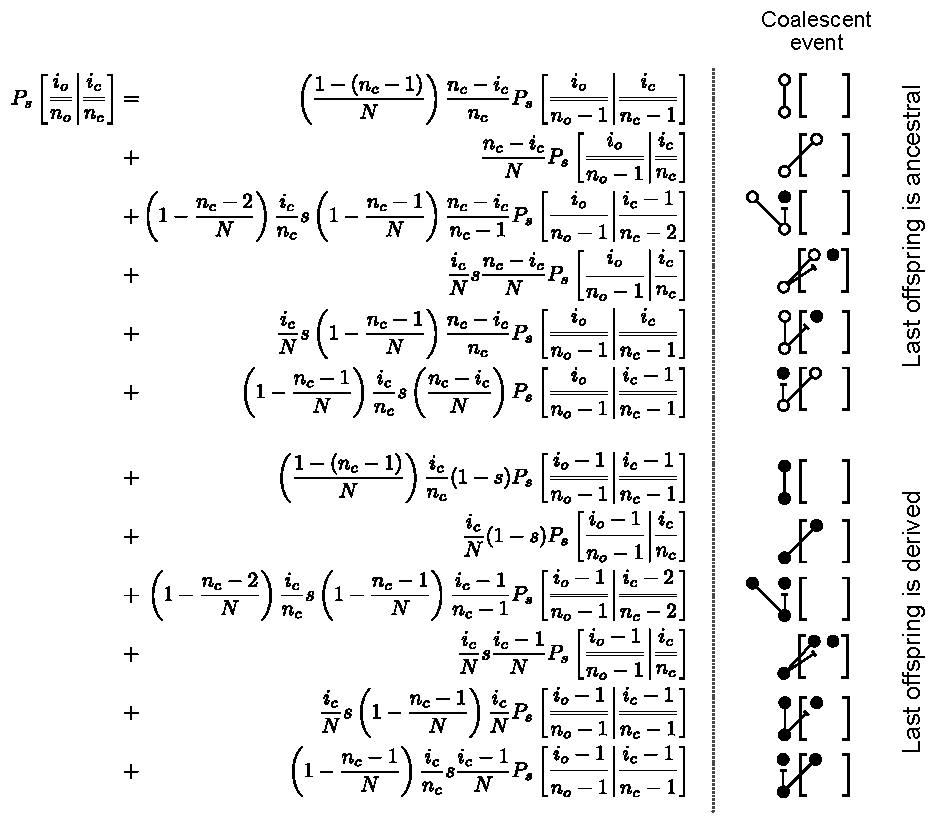
\includegraphics[width=0.9\textwidth]{fig/recurrence-selection-annotated.pdf}
%   \caption{Recurrence defining transition probabilities in a model with selection \sgcomment{I think
%       there are some problems with the way fractions are defined, e.g. the first term should start
%       with $1-\frac{n_c-1}{N}$, not $\frac{1-(n_c-1)}{N}$ }. Right panel shows coalescent events
%     corresponding to each summand. Each transition probability is defined in terms of transition in
%     a smaller sample size. First six terms are conditional on the last offspring having an ancestral
%     state, last six -- derived. Filled circles -- derived alleles; empty circles - ancestral
%     alleles; square brackets -- smaller sample.}
%   \label{fig:rec-selection}
% \end{figure}

% For each calculation, the ranges of the variables are:

% \begin{equation}
%   \begin{aligned}
%     n_p &= n \\
%     i_p &\in [0, n] \\
%     n_c &\in [1, n] \\
%     i_c &\in [0, n_c] \\
%   \end{aligned}
% \end{equation}

% Note that unlike in the neutral case $n_c$ is now variable. The base cases of the recurrence are:

% \begin{equation*}
%   \begin{aligned}
%     P\left[ \Dfrac{1}{1} \cond \Dfrac{1}{1} \right] &= 1-s \\
%     P\left[ \Dfrac{0}{1} \cond \Dfrac{0}{1} \right] &= 1 \\
%     P\left[ \Dfrac{1}{1} \cond \Dfrac{2}{2} \right] &= s \\
%     P\left[ \Dfrac{0}{1} \cond \Dfrac{1}{2} \right] &= \frac{1}{s} \\
%     \text{otherwise} &\phantom{{}=} 0
%   \end{aligned}
% \end{equation*}

\end{document}
